\documentclass[10pt,a4paper]{article}
\usepackage[spanish]{babel}
\usepackage{lmodern}
\usepackage[T1]{fontenc}
\usepackage[utf8]{inputenc}
\usepackage{amsmath}
\usepackage{amsfonts}
\usepackage{amssymb}
\usepackage{amsthm}
\usepackage{graphicx}
\usepackage{authblk}

\title{Notas de Geometría Proyectiva}
\author[1]{Nicolas Cuervo Ovalle\thanks{n.cuervo10@uniandes.edu.co}}
\author[2]{David Cardozo Bolívar\thanks{gd.cardozo684@uniandes.edu.co}}
\affil[1]{Departamento Matematicas, Universidad de los Andes}
\affil[2]{Departmento Física, Universidad de los Andes}

\renewcommand\Authands{ and }



\newtheorem{name}{Printed output}
\newtheorem{mydef}{Definición}
\newtheorem{prop}{Propiedad}


\begin{document}

\maketitle
%\makeindex
%\abstractname{temporal}%%
%com%
\section{Introducción}

La finalidad de este texto es hacer un breve recorrido sobre que es la geometría proyectiva y analizar sus propiedades.
\subsection{Historia}

Antes de entender que es la geometría proyectiva y analizar sus propiedades, es bueno introducir una breve reseña historia sobre cuales fueron los motivos que dieron origen a esta geometría. 

La geometría proyectiva tiene un origen conceptual, en el arte de perspectiva (que tuvo sus inicios a mediados del $1400$) el cual se define como `` \ldots la representación de objetos tridimensionales en una superficie bidimensional (plana) con la intención de recrear la posición relativa y profundidad de dichos objetos \ldots '' Es decir, este es un arte el cual intenta representar en un plano bidimensional la profundidad y posición relativa de los objetos en el espacio tridimensional, a su vez, este arte se caracterizo por la existencia de un punto en el `` horizonte '' o `` infinito '' en donde dos o más lineas paralelas siempre se intersectan, dicho punto lo llamamos \textit{punto de fuga}. 

\begin{figure}[h!]
    \centering
    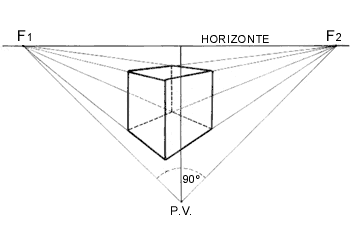
\includegraphics[scale=0.5]{imagen1.png}
    \caption{Puntos en el horizonte}
\end{figure}



Inspirado por el concepto de `` perspectiva '' el matemático francés Gerard Desaurges, conocido como el padre de la geometría proyectiva, en $1636$ escribe \textit{Traité de la perspective} el cual es conocido por ser el primer estudio conciso sobre la perspectiva y sus propiedades, planteando así por primera vez el concepto de \textit{transformación proyectiva} y asimismo introducir la idea de \textit{Geometría Proyectiva}.

\subsection{Conocimientos Previos}

Apesar de que el contenido de este texto no pretenderá ser demasiado sofisticado, es necesario definir la terminología de Campo,  Espacio Vectorial, Relación Equivalencia, Transformación Lineales, y Proyecciones sobre sub-espacios; los cuales serán necesarios para definir y entender el concepto de \textit{Geometría Proyectiva}. 


\begin{mydef} 
Un \textit{campo} (o un cuerpo) es un conjunto $ \mathbb{F} $ con dos funciones $ ( \cdot , + )$ y dos elementos distinguidos $ 1 $ y $ 0 $, ambos en $ \mathbb{F} $ tales que para todo elemento $a,b,c \in \mathbb{F}$ cumple que:

\begin{enumerate}
\item Suma
\begin{align*}
+:\mathbb{F} \times \mathbb{F} \longrightarrow \mathbb{F} \\
(a,b) \rightarrow a+b
\end{align*}

Con las siguientes propiedades:
\begin{description}

\item[Conmutativo] $a+b=b+a$
\item[Asociativo] $(a+b)+c=a+(b+c)$ 
\item [Identidad] $a+0=a$ 
\end{description}

\item Multiplicación

\begin{align*}
\cdot:\mathbb{F} \times \mathbb{F} \longrightarrow \mathbb{F} \\
(a,b) \rightarrow a \cdot b
\end{align*}

Con las siguientes propiedades:
\begin{description}
\item[Conmutativo] $a \cdot b = b \cdot a$
\item[Asociativo] $(a \cdot b) \cdot c = a \cdot (b \cdot c)$
\item [Identidad] $a \cdot 1 = a$
\item[Existencia de Inversos] $\exists \alpha \in \mathbb{F}$ tales que $a+\alpha=0$ y si $a \neq 0, \exists \beta$ tales que $a \cdot \beta = 1 $ 
\item[Distribución de $\cdot$ sobre $+$] $a \cdot (b+c) = a \cdot b + a \cdot c$
\end{description}

Por ultimo, estudiaremos sobre campos que tienen esta característica: $0 \neq 1 $


\end{enumerate}


\end{mydef}

\begin{prop}[Unicidad de Inversos] Sea $\mathbb{F}$ un campo y a $\in \mathbb{F}$ tales que existen $ \alpha,\beta \in \mathbb{F}$ tales que  $a+\alpha=0$ y si $a \neq 0, a \cdot \beta = 1 $, entonces $\alpha,\beta$ son únicos.
\end{prop}

\begin{proof}

Sea $\alpha, \alpha' \in \mathbb{F}$ tales que $a+\alpha=0$ y $a+\alpha'=0$, 
Luego,
\begin{align*}
a+\alpha= a+\alpha' \\
\Leftrightarrow a-a+\alpha = a+\alpha'-a \\
\Leftrightarrow 0+\alpha = 0+\alpha' \\
\Leftrightarrow \alpha = \alpha'
\end{align*}
Ahora sea $\beta, \beta' \in \mathbb{F}$ y  $a \neq 0$  tales que $a \cdot \beta = 1 $ y  $a \cdot \beta' = 1 $
Luego,
\begin{align*}
 a \cdot \beta = a \cdot \beta' \\
 \Leftrightarrow (a \cdot \beta)-(a \cdot \beta')=0 \\
 \Leftrightarrow a \cdot(\beta - \beta')=0 \\
\end{align*}
Como $a$ es diferente del elemento $0$, tenemos:
\begin{align*}
\Leftrightarrow \beta - \beta' = 0 \\
\Leftrightarrow \beta = \beta'
\end{align*}
Concluimos entonces, que $ \alpha $ y $ \beta $ son únicos. 

\end{proof}



\begin{mydef} Un \textit{Espacio Vectorial} sobre un campo $\mathbb{F}$ consiste de un conjunto $V$ (cuyos elementos se llaman vectores)  que consta con la operaciones de $(\cdot, +)$ anteriormente descritas junto con otra operación de múltiplos por escalares que cumple los siguientes propiedades: 
\end{mydef}

Para todo elemento $\vec{a},\vec{b},\vec{c} \in V$ se cumple que:

\begin{enumerate}
\item Suma
\begin{align*}
+: V \times V \longrightarrow V \\
(\vec{a},\vec{b}) \rightarrow \vec{a}+\vec{b}
\end{align*}
Con las siguientes propiedades:
\begin{description}
\item[Conmutativo] $\vec{a}+\vec{b}=\vec{b}+\vec{a}$
\item[Asociativo] $(\vec{a}+\vec{b})+c=\vec{a}+(\vec{b}+\vec{c})$ 
\item [Identidad] $\vec{a}+0=\vec{a}$ 
\end{description}
\item Multiplicación escalar
\begin{align*}
\cdot: V \times V \longrightarrow V \\
(\vec{a},\vec{b}) \rightarrow \vec{a}+\vec{b}
\end{align*}
Con las siguientes propiedades, para todo $ \lambda, \mu \in \mathbb{F}$: 
\begin{description}
\item $1 \cdot \vec{a} = \vec{a}$
\item $\lambda \cdot ( \mu \cdot \vec{a} ) = ( \lambda \cdot \mu ) \cdot \vec{a}  $ 
\item $ ( \lambda +  \mu ) \cdot \vec{a}  = ( \lambda \cdot \vec{a} ) + ( \mu \cdot \vec{a} )  $ 
\item $ \lambda  \cdot ( \vec{a} + \vec{b} )  = ( \lambda \cdot \vec{a} ) + ( \lambda \cdot \vec{b} )  $ 
\end{description}
\end{enumerate}

Definimos ahora el concepto de \textit{Relación}.

\begin{mydef} Sea $ A, B $ dos conjuntos no nulos, una \textit{Relación} es un conjunto $R$ tal que $ R \subseteq A\times B$ 
\end{mydef}
Dentro del conjunto de  posibles relaciones existen unas que serán vitales para nuestro estudio de geometría proyectiva. 
\begin{mydef} Una \textit{Relación de Equivalencia} es una relación $\sim$ sobre un conjunto $A$ tales que $\sim$ es reflexiva, simétrica y transitiva, es decir, para todo elemento $a,b,c \in A$:
\begin{itemize}
\item Reflexiva $ a \sim a$
\item Simétrica Si $ a \sim b \Rightarrow b \sim a$
\item Transitiva Si $a \sim b$ y $ b \sim c \Rightarrow a \sim c $
\end{itemize}
\end{mydef}
 
 
 
 
 \subsubsection{Transformación Lineal}
 
 \textit{Definición}: Sea U y V dos espacios vectoriales sobre $\mathbb{F}$. Una función(Transformación) $T:U \rightarrow V$ se denomina \textit{Lineal} si verifica: 
 
 \begin{itemize}
 \item $T(u+u')= T(u)+T(u')$ para cualquier $ u,u'\in U$
 \item $T(ku)=kT(u)$ para cualquier $u \in U$ y $k \in \mathbb{F}$
 \end{itemize}
 
 \subsubsection{Proyección}
 \textit{Definición}: Sea V un espacio vectorial sobre $\mathbb{F}$ y sean W,W' sub espacios vectoriales de V tales que $V=W\oplus W'$. La transformación lineal $P:V \rightarrow V$ definida por $P=Id(W)\oplus 0 \cdot W' $ se denomina \textit{Proyección} de W a lo largo de W'.
\textit{Nota: Se asume que el lector esta familiarizado con la terminología de subespacio vectorial y suma directa de subespacios}.
\\
\textit{Observación: si $v \in V $ es tal que $v=w+w'$ con $w \in W $ y $w' \in W'$ entonces $P(v)=P(w+w')=w$}.

\section{Geometría Proyectiva}

\subsection{Espacio Proyectivo}

Sea V un espacio vectorial sobre $\mathbb{F}$. Defina la relación de equivalencia $\sim$, donde $\forall v,w \in V, v \sim w \leftrightarrow v=\lambda \cdot w, \lambda \neq 0 $ para algún $\lambda  \in \mathbb{F}$.

\textit{Definición}: El \textit{espacio proyectivo} denotado por P(V) es el espacio cociente definido por:
\begin{align*}
P(V)= V/      \lbrace0\rbrace \setminus \sim
\end{align*}

\textit{observación}: Los elementos de P(V) son ``rectas''. (espacios 1-dimensional).
\\
\\
Ahora sea $A: V \rightarrow V $ un operador lineal invertible.
Defina $A^{*}: P(V) \rightarrow P(V)$ tales que $A^{*}([v])=[Av]$ para $v \in V$ y $[v] \in P(V)$ como una \textit{Transformación Proyectiva}. El conjunto de todas las transformaciones proyectivas es un grupo, el cual tiene por nombre el \textit{Grupo de Transformaciones Proyectivas} y lo denotaremos por GL(P). 
\\
\\
\textit{Definición}: El espacio proyectivo junto con el grupo de transformaciones proyectivas (P(V),GL(P)) se denomina \textit{Geometría Proyectiva}.

\subsection{La recta proyectiva}

\textit{Definición}: La \textit{recta proyectiva} denotada por $\mathbb{P}^{1}$ es el conjunto definido por:
\begin{align*}
\mathbb{P}^{1} := \lbrace(x,y) \in \mathbb{R}^{2} | (x,y) \neq (0,0)\rbrace \setminus \sim
\end{align*}
\textit{Recuerde}: $(x_{0},y_{0})\sim (x,y) \leftrightarrow \exists \lambda \neq 0$ tales que $\lambda(x_{0},y_{0})=(x,y)$
\\
\\
\textit{Notación}: Denotaremos a la clase de equivalencia $[(x,y)]_{\sim} \in \mathbb{P}^{1}$ por $(x:y)$
\textit{Ejemplo}: $(2:5)=(4:10)=(\dfrac{2}{5}:1)$
\\
\\
\textit{Observación}: El lector se dará cuenta que los puntos pertenecientes a la recta proyectiva son en realidad subespacios de dimensión igual a 1, es decir los puntos en la recta proyectiva realmente son rectas. De esta manera se puede entender la recta proyectiva como un circulo entendido como $\mathbb{R}\cup \lbrace\infty\rbrace$ donde esa unión de un punto ``infinito'' a los reales puede entenderse como el punto de fuga en el arte de perspectiva, de tal manera que dos puntos proyectivos se intersectan en el infinito.


\begin{figure}[h!]
    \centering
    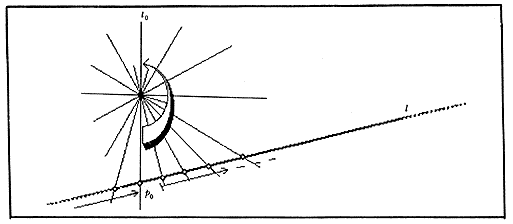
\includegraphics[scale=0.5]{imagen2.png}
    \caption{Circulos con infinitos}
\end{figure}






\subsection{El Plano Proyectivo}

\textit{Definición}: El \textit{plano proyectivo} denotado por $\mathbb{P}^{2}$ es el conjunto definido por:
\begin{align*}
 \mathbb{P}^{2} := \lbrace (x,y,z) \in \mathbb{R}^{3} | (x,y,z) \neq (0,0,0) \rbrace \setminus \sim 
\end{align*}
\textit{Notación}: Denotaremos a la clase de equivalencia $[(x,y,z)]_{\sim} \in \mathbb{P}^{2}$ por $(x:y:z)$
\\
\\
\textit{Observación}: Tomemos la esfera $\mathbb{S}^{2}$ definida por $x^2+y^2+z^2=1$, entonces cada subespacio $ \lbrace \lambda v \rbrace $ con $v \in V$ y unitario, se encuentra con la esfera en los puntos $\pm v$. Entonces 
\begin{align*}
  \mathbb{R}^{3}/\lbrace v \sim \lambda v \rbrace \cong \mathbb{S}^{2}/ \lbrace v \sim \pm v \rbrace
\end{align*} 

Luego tomemos hemisferios $\mathbb{S}^{2}_{+} = \lbrace (x,y,z) \in \mathbb{R}^{3} | z \geq 0 \rbrace$. Cada  subespacio $ \lbrace \lambda v \rbrace $ con $v = (x,y,z) con z > 0 $ se encuentra con $\mathbb{S}^{2}_{+}$ en un punto, pero los subespacios con $v = (x,y,0)$ tienen dos puntos de intersección con el hemisferio. Por lo tanto tenemos que 
\begin{align*}
\mathbb{P}^2 = \mathbb{S}^{2}/ \lbrace (x,y,0) \sim (-x,-y,0)\rbrace
\end{align*} que es equivalente a un disco con los puntos opuestos de la frontera pegados. Cabe resaltar que el proceso anterior fue la construcción geométrica del plano proyectivo donde fue necesaria la \textit{cinta de Moebius} por lo se concluye que plano no es orientable.
%(esta observacion es una cita del misha)
\\
\\ \textit{Propiedad}: En el plano proyectivo todas las \textit{secciones cónicas} son iguales.
\begin{align*}
Ax^2+2Bxy+Cy^2+2Dx+2Ey+F=0 
\end{align*}con det$\lbrace \lbrace A,B \rbrace,\lbrace D,C\rbrace \rbrace \neq 0$, son tres representaciones de la misma curva.

\section{Aplicaciones de la Geometría Proyectiva}

\subsection{Aplicación en la Teoría de Números (Ternas Pitagóricas):}

\textit{Definición}: Sea $(a,b,c) \in \mathbb{Z}^{3}$ tales que $a^2+b^2=c^2$ decimos que $(a,b,c)$ es una \textit{terna pitagórica}, si $(a,b)=(a,c)=(b,c)=1$ ( nos referimos a (x,y) como \textit{máximo común divisor de x} y \textit{y} ) decimos que la terna es \textit{primitiva}.
\\
Para encontrar las ternas pitagóricas es necesario plantear la \textit{proyección estereográfica}. Tome la ecuación de la recta que pasa por $(0,y_{0})$ y $(1,0)$ que es $-y_{0}=\dfrac{y}{x-1}$ o equivalentemente $(1-x)y_{0}=y$. 


\begin{figure}[h!]
    \centering
    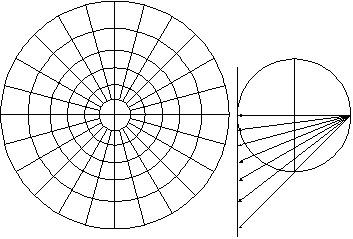
\includegraphics[scale=0.5]{imagen3.png}
    \caption{Imagen 3}
\end{figure}


De esta manera buscamos  $(x,y)$ tales que $x^2+y^2=1$, es decir $y^2=1-x^2$ remplazando en la ecuación de la recta anteriormente definida, $(1-x^2)y_{0}^{2}=1-x^2$, por medio de despejes algebraico concluimos que: 
\begin{align*}
 x_{\pm} = \dfrac{y^{2}_{0}-1}{{y^{2}_{0}+1}}  ,
 y_{\pm}=\dfrac{2y_{0}}{{y^{2}_{0}+1}} 
\end{align*}
 De esta manera definimos la \textit{proyección estereográfica} como una función de $\mathbb{R} \rightarrow \mathbb{R}^{2}$
definida por
\begin{align*}
P(T) = ( \dfrac{T^{2}-1}{T^{2}+1},\dfrac{2T}{T^{2}+1} )
\end{align*} 
\textit{Nota}: Tener solución en $x^2+y^2=z^2$ es tener solución para $(\dfrac{x}{z})^2+(\dfrac{y}{z})^2=1$
\\
\\
\textit{Observación}: Se puede observar que la proyección estereográfica tiene un parentesco con la recta proyectiva en donde el punto de fuga o infinito en este caso es el punto (1,0) como se pudo observar en la imagen. De esta manera, se puede extender el mapa anterior al espacio proyectivo. 
\\
\\ 
Considere el mapa de $\mathbb{R} \rightarrow \mathbb{R}^2 \rightarrow \mathbb{P}^2$ definido por:
\begin{align*}
 T \rightarrow (\dfrac{T^{2}-1}{T^{2}+1},\dfrac{2T}{T^{2}+1}) \rightarrow (\dfrac{T^{2}-1}{T^{2}+1}:\dfrac{2T}{T^{2}+1}:1)
\end{align*}
\\
De esta manera si toma a $T= \dfrac{s}{t}$ tenemos:
\begin{align*}
\dfrac{s}{t} \rightarrow (\dfrac{(\dfrac{s}{t})^{2}-1}{(\dfrac{s}{t})^{2}+1},\dfrac{2(\dfrac{s}{t})}{(\dfrac{s}{t})^{2}+1}) \rightarrow (\dfrac{(\dfrac{s}{t})^{2}-1}{(\dfrac{s}{t})^{2}+1}:\dfrac{2(\dfrac{s}{t})}{(\dfrac{s}{t})^{2}+1}:1)
\end{align*}
donde
\begin{align*}
(\dfrac{(\dfrac{s}{t})^{2}-1}{(\dfrac{s}{t})^{2}+1}:\dfrac{2(\dfrac{s}{t})}{(\dfrac{s}{t})^{2}+1}:1)\\
=((\dfrac{s}{t})^{2}-1:2(\dfrac{s}{t}):(\dfrac{s}{t})^{2}+1))\\
=(s^2-t^2:2st:s^2+t^2)
\end{align*}
De esta manera tenemos una extension de la \textit{proyección estereográfica} al \textit{plano proyectivo} dando paso al siguiente teorema.
\\

\textit{Teorema}: Sea $(x,y,z) \in \mathbb{Z}^3$, $(x,y,z)$ es una  \textit{terna pitagórica} con $x$ impar si y solamente si existen $(x,t) \in \mathbb{Z}^2$ tales que $(s,t)=1$; $s,t$ tienen paridad diferente con $s>t$ y $x=s^2-t^2, y=2st, z=s^2+t^2$

\textit{Nota}: La demostración de este teorema no se hará en este texto debido a que no es en base a la tesis principal del texto.  




\end{document}
